\doublespacing % Do not change - required

\chapter{Requirements and Design}
\label{ch:requirements}
\label{ch:design}

%%%%%%%%%%%%%%%%%%%%%%%%%%%%%%%%%%%%%%%
% IMPORTANT
\begin{spacing}{1} %THESE FOUR
\minitoc % LINES MUST APPEAR IN
\end{spacing} % EVERY
\thesisspacing % CHAPTER
% COPY THEM IN ANY NEW CHAPTER
%%%%%%%%%%%%%%%%%%%%%%%%%%%%%%%%%%%%%%%

This chapter turns the motivation of Chapter~\ref{ch:introduction} into a specification and then into a design. It sets out who the deliverable is for, what it must do and the constraints it must respect, and then explains the architecture, loss and evaluation choices that follow from those requirements. The as-built configuration and the measured numbers are given in Chapter~\ref{ch:implementation}, and the requirements defined here are revisited in the critical evaluation of Chapter~\ref{ch:evaluation}.

\section{Intended Use}
\label{sec:req_stakeholders}

The deliverable is a NIR$\rightarrow$RGB pre-processor, a module placed between a near-infrared sensor and an existing RGB-trained vision model. Its user is an engineer who already has a working RGB perception stack, such as an object detector, a segmentation network or a depth model, and a reason to run it on NIR input such as night operation, biometric imaging or material inspection.

The direct alternative is to retrain or fine-tune each downstream model on NIR data, but this is often impractical. It needs the model weights to be openly available, and it needs a large amount of NIR data to be collected and labelled for every task. A single translator that restores RGB-like performance avoids most of this cost and leaves each downstream model unchanged.

\section{Functional Requirements}
\label{sec:req_functional}

\begin{enumerate}
    \item \textbf{F1: Translation.} Map a 3-channel NIR image to a 3-channel RGB image of the same scene at the same resolution.
    \item \textbf{F2: Geometry preservation.} Preserve spatial structure. Object boundaries, thin structures and positions must not move, so that a downstream model's spatial outputs remain valid.
    \item \textbf{F3: Determinism.} Produce the same output for the same input. As a stage in a perception pipeline, stochastic output would inject noise into every downstream model.
    \item \textbf{F4: Drop-in interface.} Accept the sensor's native frames and produce standard 8-bit RGB, so the downstream model is used unmodified.
\end{enumerate}

\section{Non-Functional Requirements}
\label{sec:req_nonfunctional}

\begin{enumerate}
    \item \textbf{N1: Throughput.} Run at an interactive frame rate of around 5\,FPS, roughly 200\,ms per frame, at the deployment resolution on the target Raspberry~Pi~5 CPU.
    \item \textbf{N2: Edge footprint.} Fit within the compute and memory budget of the target device after INT8 quantisation. The deployed model must load and run without swapping or an out-of-memory failure while meeting N1. Artefact size and peak resident memory are reported for the distilled student of Section~\ref{sec:edge_student}.
    \item \textbf{N3: Quality measured by downstream utility.} Judge success by how much downstream-task performance is recovered relative to native RGB, the gap-closure metric of Section~\ref{sec:design_evaluation}, rather than by pixel fidelity such as PSNR alone.
\end{enumerate}


\section{Design Goals}
\label{sec:design_goals}

The requirements lead to four design drivers, which together point to a single class of solution.

\begin{itemize}
    \item \textbf{Semantic preservation over photorealism.} The output is consumed by frozen RGB-pretrained models, not by human viewers, so edges, boundaries, thin structures and material identity matter more than absolute colour accuracy. This follows from F2 and N3.
    \item \textbf{Deterministic, low-latency inference.} The translator must give the same output for the same input and run in a small, predictable per-frame budget. This follows from F3 and N1.
    \item \textbf{Edge deployment on the Raspberry~Pi~5.} This rules out architectures whose operators are unsupported by the chosen Pi~5 runtime, and any whose compute or memory footprint exceeds what the device can sustain in real time. This follows from N1 and N2.
    \item \textbf{Paired supervision from a small bespoke dataset.} Public RGB--NIR pairs are limited and often imperfectly aligned, as discussed in Section~\ref{sec:datasets}, so a dedicated capture rig is required.
\end{itemize}

Together these favour a deterministic, supervised feed-forward translator with strong structural regularisation. This excludes both an unpaired CycleGAN-style approach and a stochastic diffusion model. The rest of the chapter works through the architecture, loss and evaluation choices that follow.

\section{Semantic Preservation and ``Semantic Drift''}
\label{sec:semantic_drift}

Image-to-image translation can lose semantics during conversion. Even a photorealistic output may move object boundaries, drop small but meaningful structures, or hallucinate edges and textures that were not in the input. NIR-to-RGB is especially exposed to this because the model must also infer colour. Where the training data correlates particular materials or backgrounds with particular colours, the generator can over-rely on those priors and alter the scene in semantically important ways.

This semantic drift matters most when translated images feed downstream tasks such as detection, segmentation and identity recognition, where small geometric warps, boundary shifts or spurious high-frequency detail hurt performance more than colour errors do. The standard mitigations are reviewed in Sections~\ref{sec:pix2pixhd} and~\ref{sec:pix2next}. The decision taken here is to push that idea further and supervise on the deep features the downstream models actually use, as set out in the loss design of Section~\ref{sec:loss_design}.  \autoref{fig:pix2pix_semantic_drift} shows it observed directly in an early experiment for this project, in which a pix2pix model trained on the KAIST thermal benchmark fails to preserve a roadside sign that is clearly visible in the input.

\begin{figure}[!htbp]
    \centering
    \begin{minipage}{0.31\textwidth}
        \centering
        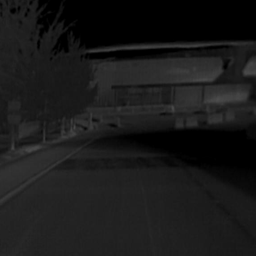
\includegraphics[width=\linewidth]{imgs/pix2pix-poor-semantic-result/IR-image.png}
        \subcap{(a) LWIR input}
    \end{minipage}\hfill%
    \begin{minipage}{0.31\textwidth}
        \centering
        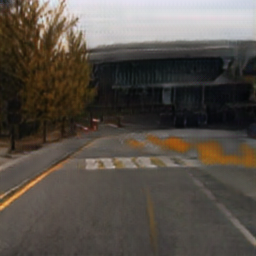
\includegraphics[width=\linewidth]{imgs/pix2pix-poor-semantic-result/RGB-fake.png}
        \subcap{(b) pix2pix output}
    \end{minipage}\hfill%
    \begin{minipage}{0.31\textwidth}
        \centering
        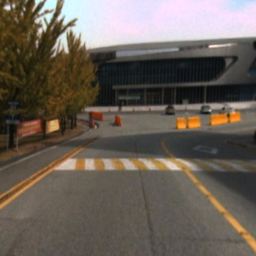
\includegraphics[width=\linewidth]{imgs/pix2pix-poor-semantic-result/RGB-real.png}
        \subcap{(c) Ground-truth RGB}
    \end{minipage}
    \caption{Example of semantic drift in long-wave infrared (LWIR)$\rightarrow$RGB translation, produced by a pix2pix model trained for this project on the KAIST RGB--thermal benchmark~\cite{hwang2015multispectral}}
    \label{fig:pix2pix_semantic_drift}
\end{figure}

\section{Architecture Choice}
\label{sec:architecture_choice}

Two architecture families were considered.

\begin{description}
    \item[Pix2Pix U-Net (baseline).] A Pix2Pix-style 8-level U-Net generator with a PatchGAN discriminator is the canonical paired-translation baseline~\cite{isola2017image} and the formulation most later paired-translation methods build on, which makes it a strong and fair point of comparison. Its strengths are sharp output, simple training and easy export, and its weaknesses are well documented: it is BatchNorm-heavy, has around 54\,M parameters at base width 64, and is prone to semantic drift under one-to-many ambiguity.
    \item[NAFNet teacher (selected).] NAFNet~\cite{chen2022nafnet} is a modern simple-baselines architecture for image restoration. Compared to the Pix2Pix U-Net it has no nonlinear activations, using a SimpleGate and channel attention instead, which gives stable training and predictable INT8 quantisation. Its layer-normalised blocks behave well at small batch sizes, and its pure-CNN structure exports cleanly to ONNX and the common Pi~5 runtimes such as ONNX Runtime, NCNN and TFLite. The teacher uses the width-64 configuration, with $[2,2,4,8]$ encoder blocks and 12 middle blocks, for around 116\,M parameters. The as-built model is detailed in Section~\ref{sec:nafnet_teacher}.
\end{description}

\subsection{Edge Student}
\label{sec:edge_student}

The NAFNet teacher is large because it is not the deployed model. A smaller width-16 NAFNet, with reduced width and block depth, is distilled from it and quantised to INT8 for the Raspberry~Pi~5 CPU, as described in Section~\ref{sec:edge_deployment}. Separating teacher from student lets the teacher train at full quality on a desktop GPU while the student is shaped to the latency and memory budget of the deployment target.

\section{Loss Design}
\label{sec:loss_design}

The starting point is the standard objective for paired image translation: an L1 reconstruction term for colour fidelity, a VGG-16 perceptual term for feature-space similarity~\cite{johnson2016perceptual}, a least-squares PatchGAN term for local realism, and a multi-scale SSIM term for structural fidelity~\cite{wang2003msssim}.

The central design decision of this project is to change what the perceptual supervision matches. Because the translated image is consumed by frozen RGB-pretrained networks rather than by a human, the objective that best serves the goal is agreement in the deep-feature spaces those networks use, which is the quantity the downstream evaluation measures in Section~\ref{sec:design_evaluation}. A single ImageNet-VGG perceptual term captures only one such space. The final teacher therefore replaces it with a set of frozen foundation models: DINOv2~\cite{oquab2024dinov2} for self-supervised features, CLIP~\cite{radford2021clip} for vision--language features, and ResNet-50~\cite{he2016resnet} for ImageNet-supervised features. Matching features across this ensemble pushes the output to sit within the input distribution of many representations rather than one, as a task-agnostic pre-processor requires.

Formally, writing $T$ for the translator and $F$ for a frozen feature extractor, training pushes $F(T(x_{\text{NIR}})) \approx F(x_{\text{RGB}})$ for each $F$ in the ensemble, so a downstream model whose predictions depend on $F(\cdot)$ behaves on $T(x_{\text{NIR}})$ more like it does on $x_{\text{RGB}}$. The gap-closure metric of Section~\ref{sec:design_evaluation} measures empirically how well this holds for each downstream task.

The final recipe keeps the stabilising parts of the conventional objective: a strong L1 colour anchor, an MS-SSIM structural term and a lightly weighted PatchGAN term. The VGG perceptual term is dropped, since it captures only one ImageNet feature space, and the foundation ensemble supplies the task-facing perceptual signal in its place. The exact weights are given in Section~\ref{sec:nafnet_teacher} and \autoref{tab:teacher_loss}.

\section{Why Not Diffusion or Bridge Models?}
\label{sec:why_not_diffusion}

Conditional diffusion and bridge models (Section~\ref{sec:i2i_diffusion}) represent the one-to-many ambiguity of NIR$\rightarrow$RGB colourisation well, but they were rejected on two grounds. Sampling requires many denoising steps, which is incompatible with the 200\,ms-per-frame target on the Raspberry~Pi~5, where a single forward pass through a NAFNet student is comparable in cost to one diffusion step. And their sampling is stochastic, which violates the determinism requirement F3 by construction. Schr\"odinger-bridge formulations remain interesting for offline data augmentation, for example synthesising additional NIR/RGB pairs from one-sided data, but not for deployment.

\section{Evaluation Design}
\label{sec:design_evaluation}

Standard image-quality metrics such as PSNR, SSIM and LPIPS measure how close the translated RGB is to ground-truth RGB. They do not measure whether downstream pretrained models work better on the translated image, which is this project's goal. To address this, a downstream evaluation harness was designed. It runs a panel of frozen RGB-pretrained networks on three inputs, raw NIR, translated RGB and ground-truth RGB, and reports a per-task \emph{gap closure}
\[
\text{gap\_closure} \;=\; \frac{m(\text{translated}) - m(\text{nir})}{m(\text{rgb}) - m(\text{nir})}
\]
where $m(\cdot)$ is the primary metric of the downstream task, for example matched detection Intersection over Union (IoU) or semantic-segmentation mean IoU (mIoU). A value of 0 means the translation is no better than raw NIR, 1 means native-RGB behaviour is fully recovered and a negative value means the translation made the task worse than raw NIR. For metrics where lower is better, such as the per-image normalised depth error used in Chapter~\ref{ch:results}, $m(\cdot)$ is defined so that the sign convention above still holds, with the harness inverting the raw difference accordingly. Full results are reported in Chapter~\ref{ch:results}.

\section{Success Criteria and Risk Register}
\label{sec:req_success}

The project is successful if it meets three criteria. S1, a paired and geometrically aligned NIR/RGB dataset is collected at sufficient scale for supervised training. S2, the translator yields positive gap closure on a majority of the downstream panel, at least three of the five tasks, with no task driven below its raw-NIR baseline. S3, the deployed student meets the 5\,FPS throughput target of N1 on the Pi~5. The quantitative thresholds and the final scoring against these criteria are reported in Chapters~\ref{ch:results} and~\ref{ch:evaluation}.

The main risks to these outcomes, and the design choices that mitigate them, are summarised in \autoref{tab:risk_register}.

\enlargethispage{3\baselineskip}
\begin{table}[!htbp]
\centering
\footnotesize
\begin{tabular}{p{0.30\linewidth}p{0.60\linewidth}}
\hline
\textbf{Risk} & \textbf{Mitigation} \\
\hline
Imperfectly aligned NIR/RGB pairs corrupt supervision (S1) & Shared-aperture capture rig, so each pair is simultaneous and related by a single depth-independent homography (Section~\ref{sec:datasets}). \\
Semantic drift toward dataset-average colour (S2) & Feature-space supervision against a foundation ensemble, with evaluation on downstream tasks rather than pixel fidelity (Sections~\ref{sec:loss_design} and~\ref{sec:design_evaluation}). \\
Student misses the latency budget on the Pi~5 (S3) & Width-16 distilled student, INT8 quantisation, and selection of the fastest supported runtime (Section~\ref{sec:edge_deployment}). \\
Limited paired data leads to overfitting (S1, S2) & Data augmentation and task-agnostic foundation-feature supervision rather than reliance on one feature space. \\
\hline
\end{tabular}
\caption{Principal project risks and the design choices that mitigate them.}
\label{tab:risk_register}
\end{table}
